\section{空间中的子集}
\label{sec:topo-subsets}

固定一个拓扑空间$X$，它的子集$A$与环境之间有几种自然的关系：$A$的补集是否开放，$A$中哪些点被$A$自身围住，环境中哪些点虽不在$A$内却紧贴着$A$。这些判断都相对于给定的拓扑，换一个拓扑，同一个集合的内部和闭包都可能改变。

\subsection{闭集}
\label{sec:topo-closed-sets}

开集描述“每点都留有余地”，与之互补的是“集合外每点都留有余地”：若$x\notin F$，则$x$有一个完全落在$F$外的开邻域。这正是说$X\setminus F$是开集。

\begin{definition}[闭集]
\label{def:topo-closed-set}
拓扑空间$X$的子集$F$称为\term{闭集}（closed set），如果它的补集$X\setminus F$是开集。
\end{definition}

De Morgan律把并变成交、把交变成并，于是定义~\ref{def:topo-topology}的三条规则转为闭集的三条规则：$\varnothing$与$X$是闭集；任意多个闭集的交是闭集；有限多个闭集的并是闭集。

“有限”同样不能去掉。在$\mathbb R$中，闭区间$[1/n,1]$（$n\geq1$）的并是
\[
 \bigcup_{n\geq1}\Bigl[\frac1n,1\Bigr]=(0,1],
\]
它不是闭集，因为补集$(-\infty,0]\cup(1,\infty)$在点$0$处没有落在其中的开邻域。

\paragraph{实轴上的区间}
闭区间$[a,b]$是闭集，因为补集$(-\infty,a)\cup(b,\infty)$是两个开集的并。开区间$(a,b)$不是闭集：补集$(-\infty,a]\cup[b,\infty)$含端点$a$，而$a$的每个开邻域都与$(a,b)$相交，所以补集不开。半开区间$[a,b)$既不是开集（$a$处没有余地），也不是闭集（补集在$b$处没有余地）。

\paragraph{开与闭不是互斥的两类}
日常语言里“开”与“闭”是反义词，在拓扑中它们却是两个独立的条件。$\mathbb R$本身和空集既开又闭，$[a,b)$既不开也不闭。离散拓扑中每个子集都既开又闭，平凡拓扑中只有$\varnothing$与$X$是闭集。

所以证明一个集合“不是开集”并不能推出它是闭集。既开又闭的子集在第~\ref{sec:topo-connected-sets}小节会成为判断空间能否拆分的工具。

\subsection{内部、闭包与边界}
\label{sec:topo-interior-closure}

一个子集$A$通常既不开也不闭，例如$[0,1)$。为了描述它离“开”和“闭”各差多少，我们按每一点与$A$的关系把空间中的点分类。图~\ref{fig:topo-interior-closure}画出了平面上的三种情形：有些点被$A$完全围住，有些点无论多小的邻域都同时碰到$A$与$A$的外部，还有些点有一个完全避开$A$的邻域。

\begin{BookInlineFigure}
  \centering
  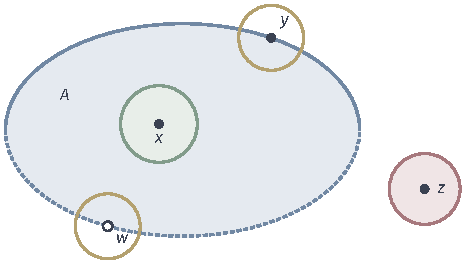
\includegraphics[width=78.807mm]{figures/04-spaces-measures-and-geometry/01-topology-and-metric/tikz/topo-interior-closure/figure.pdf}
  \caption{点与子集的三种关系。$A$是椭圆区域，实线部分的边界属于$A$，虚线部分不属于$A$。$x$有落在$A$内的邻域（绿色），是内点；$z$有与$A$不交的邻域（红色），不在闭包中；$y$与$w$的每个邻域（黄色）都既含$A$的点又含$A$外的点，二者都是边界点，其中$y\in A$，$w\notin A$。}
  \label{fig:topo-interior-closure}
\end{BookInlineFigure}

\paragraph{内部}
点$x$称为$A$的\term{内点}（interior point），如果$A$是$x$的邻域，即有开集$U$满足$x\in U\subseteq A$。$A$的全体内点组成$A$的\term{内部}（interior），记作$\operatorname{int}A$。

把每个内点的这种$U$合起来，得到$\operatorname{int}A$等于含于$A$的所有开集之并，因而它是含于$A$的最大开集。由引理~\ref{lem:topo-open-iff-neighborhood}，$A$开当且仅当$\operatorname{int}A=A$。

\paragraph{闭包}
从另一侧看，点$x$可能不在$A$中，却被$A$紧紧挨着：$x$的每个邻域都含有$A$的点。这时把$x$算作$A$能“接近”的点。

\begin{definition}[闭包]
\label{def:topo-closure}
设$A\subseteq X$。若$x$的每个邻域都与$A$相交，称$x$为$A$的\term{闭包点}（closure point）。$A$的全体闭包点组成的集合称为$A$的\term{闭包}（closure），记作$\overline A$。
\end{definition}

每个邻域都含一个开邻域，所以判断闭包点时只需检验开邻域，或者只需检验某个邻域基的成员。若$x\in A$，则$x$的每个邻域都含$x$，因而与$A$相交，所以$A\subseteq\overline A$。闭包也有一个与内部对称的刻画。

\begin{theorem}[闭包是最小闭超集]
\label{thm:topo-closure-smallest-closed}
对任意$A\subseteq X$，$\overline A$等于所有包含$A$的闭集之交。因此$\overline A$是闭集，并且是包含$A$的最小闭集；$A$闭当且仅当$\overline A=A$。
\end{theorem}
\begin{proof}
记$C$为包含$A$的所有闭集之交。若$x\notin\overline A$，则$x$有开邻域$U$与$A$不交。$X\setminus U$是包含$A$的闭集且不含$x$，所以$x\notin C$。这说明$C\subseteq\overline A$。

反过来，若$x\notin C$，则存在包含$A$的闭集$F$使$x\notin F$。$X\setminus F$是$x$的开邻域，它与$F$不交，因而与$A$不交，$x$不是闭包点。这说明$\overline A\subseteq C$。

闭集之交是闭集，所以$\overline A$闭。其余结论由“最小闭集”直接得到：$A$闭时$A$自己就是包含$A$的最小闭集。
\end{proof}

内部与闭包通过补集相互转换：$x$不是$A$的闭包点，恰好是说$x$有一个开邻域含于$X\setminus A$，即$x$是$X\setminus A$的内点。所以
\begin{equation}
 X\setminus\overline A=\operatorname{int}(X\setminus A).
 \label{eq:topo-closure-interior-complement}
\end{equation}

\paragraph{边界}
闭包与内部之差是那些既能接近$A$、又不被$A$围住的点。称
\begin{equation}
 \partial A=\overline A\setminus\operatorname{int}A
 \label{eq:topo-boundary}
\end{equation}
为$A$的\term{边界}（boundary）。由式~\eqref{eq:topo-closure-interior-complement}，$x\in\partial A$当且仅当$x$的每个邻域都既含$A$的点、又含$X\setminus A$的点。这个判据对$A$与$X\setminus A$对称，所以$\partial A=\partial(X\setminus A)$。

\begin{example}[同一集合在不同拓扑下]
\label{ex:topo-interior-closure-examples}
在$\mathbb R$的通常拓扑下取$A=[0,1)$。$(0,1)$中每点有含于$A$的小区间，$0$没有，所以$\operatorname{int}A=(0,1)$。$1$的每个邻域都含$A$中靠近$1$的点，$[0,1]$外的点有与$A$不交的邻域，所以$\overline A=[0,1]$。由式~\eqref{eq:topo-boundary}，$\partial A=\{0,1\}$。

有理数集$\mathbb Q$的内部为空，因为每个区间都含无理数。它的闭包是$\mathbb R$（见下一小节），所以$\partial\mathbb Q=\mathbb R$。

把$\mathbb R$换成离散拓扑，$A=[0,1)$既开又闭，于是
\[
 \operatorname{int}A=\overline A=A,\qquad\partial A=\varnothing.
\]

换成平凡拓扑，唯一含于$A$的开集是空集，唯一的非空开集$\mathbb R$与$A$相交，所以
\[
 \operatorname{int}A=\varnothing,\qquad\overline A=\mathbb R,\qquad\partial A=\mathbb R.
\]
\end{example}

表~\ref{tab:topo-three-topologies}把结果并排列出。同一个集合在三种拓扑下得到三组完全不同的答案，内部、闭包与边界描述的是集合在某个拓扑中的位置。

\begin{BookInlineTable}
  \centering
  \begin{tabular}{@{}llll@{}}
    \toprule
    $\mathbb R$上的拓扑 & $\operatorname{int}A$ & $\overline A$ & $\partial A$\\
    \midrule
    通常拓扑 & $(0,1)$ & $[0,1]$ & $\{0,1\}$\\
    离散拓扑 & $[0,1)$ & $[0,1)$ & $\varnothing$\\
    平凡拓扑 & $\varnothing$ & $\mathbb R$ & $\mathbb R$\\
    \bottomrule
  \end{tabular}
  \caption{集合$A=[0,1)$在三种拓扑下的内部、闭包与边界。}
  \label{tab:topo-three-topologies}
\end{BookInlineTable}

有限空间上可以完整地算一遍。取图~\ref{fig:topo-finite-topologies}(b)的拓扑，它的开集是$\varnothing,\{a\},\{a,b\},X$，取补集得到闭集
\[
 X,\quad\{b,c\},\quad\{c\},\quad\varnothing.
\]

设$A=\{b\}$。含于$A$的开集只有$\varnothing$，所以$\operatorname{int}A=\varnothing$。包含$A$的闭集是$\{b,c\}$与$X$，它们的交是$\{b,c\}$，由定理~\ref{thm:topo-closure-smallest-closed}得到
\[
 \overline A=\{b,c\},\qquad\partial A=\{b,c\}.
\]
点$c$也在闭包里，因为$c$唯一的开邻域$X$含有$b$。

在有距离的空间里，闭包点还能用“到$A$的距离为零”来刻画，这一判据依赖度量，放在第~\ref{chap:metric-spaces}章建立。

\subsection{稠密集}
\label{sec:topo-dense-sets}

每个实数都能被有理数任意接近，用闭包的语言，这就是说$\mathbb Q$的闭包是整个$\mathbb R$。把这一性质抽象出来，就是稠密。

\begin{definition}[稠密集]
\label{def:topo-dense}
若$D\subseteq X$满足$\overline D=X$，称$D$在$X$中\term{稠密}（dense）。
\end{definition}

由闭包的定义，$\overline D=X$意味着每个点的每个邻域都与$D$相交。每个非空开集都是它每个点的邻域，所以这又可以写成只涉及开集的判据。

\begin{theorem}[稠密的开集判据]
\label{thm:topo-dense-open-criterion}
$D$在$X$中稠密，当且仅当$X$的每个非空开集都与$D$相交。
\end{theorem}
\begin{proof}
设$D$稠密，$U$是非空开集，取$x\in U$。$U$是$x$的邻域，而$x\in\overline D$，所以$U\cap D\neq\varnothing$。

反过来，设每个非空开集都与$D$相交。任取$x\in X$及其邻域$N$，$N$含某个开集$U\ni x$。$U$非空，故与$D$相交，于是$N$也与$D$相交，$x\in\overline D$。
\end{proof}

\begin{example}[有理数与无理数都稠密]
\label{ex:topo-rationals-irrationals-dense}
由定理~\ref{thm:topo-dense-open-criterion}，只需证明每个开区间$(a,b)$（$a<b$）都含有理数和无理数。

由实数的Archimedes性质（由确界原理推出，可参考\BookChapterRef{chap:real-complex-functions}{卷一第4章“实数、复数与函数”}），可取正整数$n$使$1/n<b-a$，再取最小的整数$m$使$m/n>a$。由$m$的最小性，$(m-1)/n\leq a$，所以
\[
 a<\frac mn\leq a+\frac1n<b.
\]

用数字走一遍。设$(a,b)=(0.3,0.31)$，长度为$0.01$，取$n=101$。$30/101\approx0.2970$还小于$0.3$，所以$m=31$，得到
\[
 \frac{31}{101}\approx0.3069\in(0.3,0.31).
\]

对无理数，把同样的论证用于区间$(a-\sqrt2,b-\sqrt2)$，得到其中的有理数$q$，则$q+\sqrt2\in(a,b)$。$q+\sqrt2$是无理数，否则$\sqrt2=(q+\sqrt2)-q$会是有理数。所以$\mathbb Q$与$\mathbb R\setminus\mathbb Q$都在$\mathbb R$中稠密，而它们互不相交。
\end{example}

稠密并不要求子集占据大部分空间。$\mathbb Q$与无理数集都稠密，却彼此不交；第~\ref{chap:measure}章还会看到，$\mathbb Q$的长度为零。稠密只说明子集能接近空间中的每一点，并没有覆盖它们。

\paragraph{为什么不用点列定义稠密}
在$\mathbb R$中，$D$稠密等价于每个实数都是$D$中某个点列的极限。一般拓扑空间中，邻域可能多到无法用可数个依次缩小的集合代表，点列这时走不到闭包中的所有点。第~\ref{sec:topo-convergence}节将给出这样的空间，所以闭包与稠密性都以邻域定义，点列判据只在附加条件下成立。
